\documentclass[12pt,a4paper]{article}
\author{}
\date{}
\title{Mueller Plathe}
\usepackage{amsmath}
\usepackage{graphicx}
\begin{document}
\maketitle
\paragraph{} 
\begin{figure}[h]
  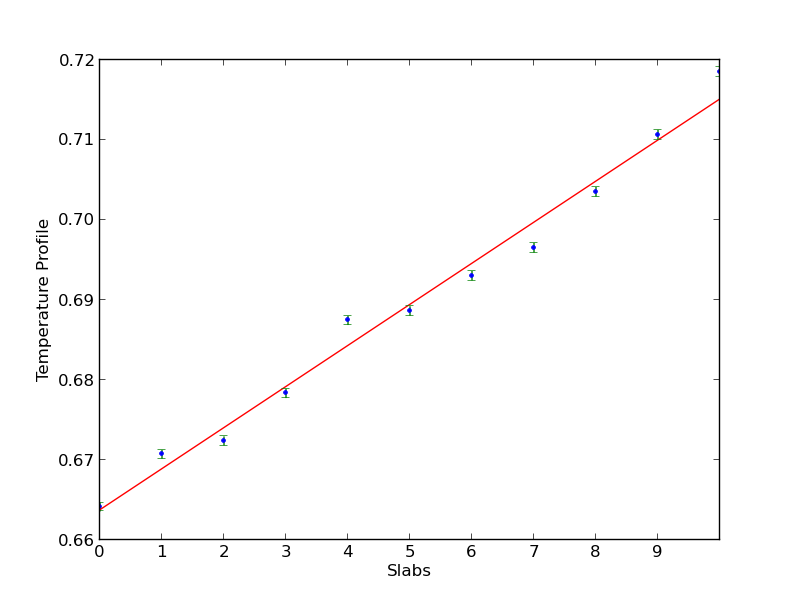
\includegraphics[width=\linewidth]{1.png}
\end{figure}

\begin{align*}
 \kappa &= 7.0507535737 \\
 \sigma_\kappa&=0.28168932463
\end{align*}
\begin{figure}[h]
  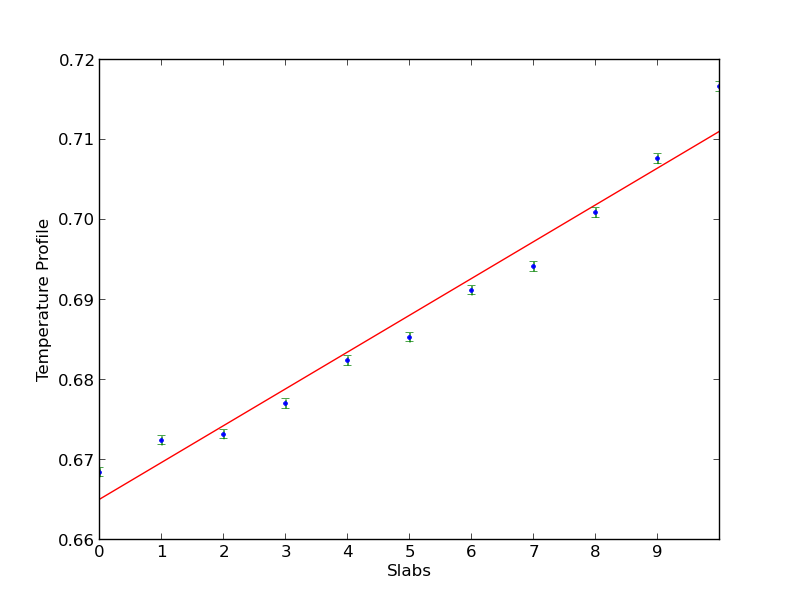
\includegraphics[width=\linewidth]{2.png}
\end{figure}
\begin{figure}[h]
  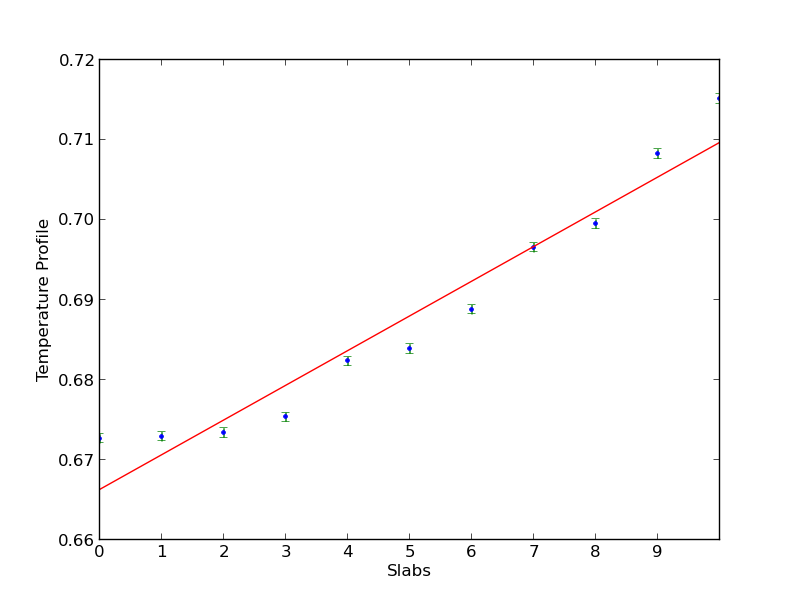
\includegraphics[width=\linewidth]{3.png}
\end{figure}
\paragraph{}
\begin{align*}
\kappa &=6.770354882  \\
\sigma_\kappa &=0.3083434129
\end{align*}

	
	\end{document}